\section{惩罚法}
\label{sec:opt-con-penalty}

上一节要求每一步都可行，这需要投影或线性子问题容易求解。约束一旦是非线性的，或可行域的投影本身就是难题，这一要求便难以满足。惩罚法换一种思路：允许迭代点暂时违约，但给违约计价，把约束问题换成一个（或一列）无约束问题，交给第~\ref{chap:opt-smooth}章和第~\ref{chap:opt-nonsmooth}章的方法求解。计价方式决定了两种不同的目标：二次惩罚只在罚参数趋于无穷时逐步逼近可行，精确惩罚则在罚参数超过某个有限阈值后就保留原问题的解。下一节的乘子法会在惩罚之外再更新乘子。

\subsection{二次惩罚法}
\label{sec:opt-con-quadratic-penalty}

\paragraph{给违约的平方计价}
用约束残差构造违约度量$P(\bm x)=\sum_jh_j(\bm x)^2+\sum_i[g_i(\bm x)]_+^2$，其中$[t]_+=\max\{t,0\}$。$P\geq0$，且$P(\bm x)=0$当且仅当$\bm x$可行。对罚参数$\rho>0$，\term{二次惩罚法}（quadratic penalty method）求解
\begin{equation}
\label{eq:opt-con-quadratic-penalty}
  \min_{\bm x}\ Q_\rho(\bm x)=f(\bm x)+\frac\rho2P(\bm x).
\end{equation}
函数$[t]_+^2$连续可微，导数为$2[t]_+$，所以$f,g_i,h_j$连续可微时$Q_\rho$也连续可微，可以用梯度类方法求解；但$[t]_+^2$在$t=0$处二阶导数跳变，牛顿法在活动集变化处可能受影响。约束仿射时罚项是凸二次函数；约束非线性时，罚项一般不继承凸性，例如$h(x)=x^2-1$的平方$(x^2-1)^2$在$x=0$附近是凹的。

罚参数在原目标与违约之间取舍。对等式二次例，$Q_\rho=\frac12(x_1^2+4x_2^2)+\frac\rho2(x_1+x_2-1)^2$，令梯度为零：$x_1+\rho r=0$、$4x_2+\rho r=0$，其中$r=x_1+x_2-1$。于是$x_1=-\rho r$、$x_2=-\rho r/4$，代回$r$的定义得$r=-\frac54\rho r-1$，即
\[
  \bm x_\rho=\frac{(4\rho,\ \rho)^\top}{4+5\rho},\qquad
  h(\bm x_\rho)=-\frac{4}{4+5\rho}.
\]
任何有限的$\rho$都给出不可行的点，违约随$\rho$增大按$1/\rho$的速度减小，$\bm x_\rho$沿一条从原点出发的射线逼近$\bm x^\star=(4/5,1/5)^\top$（图~\ref{fig:opt-con-penalty-path}(a)）。顺带还能读出乘子：驻点方程与$\nabla f+\nu\nabla h=\bm0$对照，$\rho h(\bm x_\rho)=-4\rho/(4+5\rho)$扮演乘子的角色，并随$\rho\to\infty$趋于$\nu^\star=-4/5$。这一观察是下一节增广Lagrange法的出发点。

\begin{algorithm}[二次惩罚法]
\label{alg:opt-con-quadratic-penalty}
\begin{algorithmic}[1]
\Require 初值$\bm x^{(0)}$，初始罚参数$\rho_0>0$，放大因子$\beta>1$，内层容差序列$\epsilon_k\to0$，可行性容差$\epsilon_{\mathrm{feas}}$
\Ensure 近似可行的候选$\bm x_k$
\For{$k=0,1,2,\dots$}
  \State 从上一轮的解出发（热启动），近似求解$\min Q_{\rho_k}$，直到$\lVert\nabla Q_{\rho_k}(\bm x_k)\rVert_2\leq\epsilon_k$
  \State 分别记录$f(\bm x_k)$、约束违约$\sqrt{P(\bm x_k)}$与内层精度
  \If{$\sqrt{P(\bm x_k)}\leq\epsilon_{\mathrm{feas}}$且$\epsilon_k$足够小}
    \State 返回$\bm x_k$
  \EndIf
  \State $\rho_{k+1}=\beta\rho_k$
\EndFor
\end{algorithmic}
\end{algorithm}

停止判断不能只看罚目标：$\nabla Q_\rho$很小只说明解好了罚问题，原约束是否满足、违约多大，必须按原约束单独报告。

\paragraph{可行极限与最优性}
二次惩罚何时把迭代带到原问题的解，需要把几个条件分开说明。

\begin{theorem}[二次惩罚的极限]
\label{thm:opt-con-quadratic-penalty}
设$f,g_i,h_j$连续，可行域非空，$f$在$\mathbb R^d$上有下界$m$，$\rho_k\to\infty$，且$\bm x_k$是$Q_{\rho_k}$的全局最小点。则：(1) 对任意可行$\bar{\bm x}$，$P(\bm x_k)\leq2(f(\bar{\bm x})-m)/\rho_k\to0$；(2) $(\bm x_k)$的每个极限点都是原问题的全局最小点。
\end{theorem}

\begin{proof}
由$\bm x_k$的最优性和$P(\bar{\bm x})=0$，$f(\bm x_k)+\frac{\rho_k}2P(\bm x_k)\leq f(\bar{\bm x})$。于是$f(\bm x_k)\leq f(\bar{\bm x})$，且$\frac{\rho_k}2P(\bm x_k)\leq f(\bar{\bm x})-m$，得(1)。设$\bm x_{k_l}\to\hat{\bm x}$，由$P$连续得$P(\hat{\bm x})=0$，$\hat{\bm x}$可行；由$f$连续，$f(\hat{\bm x})=\lim f(\bm x_{k_l})\leq f(\bar{\bm x})$。$\bar{\bm x}$是任意可行点，故$\hat{\bm x}$是全局最小点。
\end{proof}

定理的每个条件管一段：下界$m$控制违约；连续性把“违约趋于零”传递到极限点；“极限点存在”还需要序列有界，这要另外验证（例如$f$强制）。内层只求到$\varepsilon_k$次优时，(1)中的分子变为$f(\bar{\bm x})-m+\varepsilon_k$，$\varepsilon_k$有界即可保证违约趋于零，而(2)还需要$\varepsilon_k\to0$。实际计算中$\bm x_k$通常只是$Q_{\rho_k}$的局部最小点或驻点，此时只能期望极限点满足一阶条件，不能得到全局结论。

\paragraph{罚参数增大带来的病态}
可行性的代价是曲率失衡。等式二次例中$\nabla^2Q_\rho=\operatorname{diag}(1,4)+\rho\bm1\bm1^\top$，特征值为$\frac12\bigl((5+2\rho)\pm\sqrt{9+4\rho^2}\bigr)$。约束法向$(1,1)^\top$方向上的曲率随$\rho$线性增长，沿约束线方向的曲率却趋于常数$5/2$，条件数在$\rho=0,1,10,100$时分别约为$4$、$3.1$、$9.5$、$81$，此后约以$0.8\rho$的速度增长（起初略降，因为罚项先补足了$x_1$方向较小的曲率）。图~\ref{fig:opt-con-penalty-path}(a)中$\rho=20$时罚目标的等值线已被压成沿约束线的细长椭圆。梯度法的步长受最大曲率限制、而进展受最小曲率限制，迭代数随条件数增长；牛顿法每步要解的线性系统同样病态，舍入误差随之放大。因此外层$\rho$应逐步增大并热启动，内层容差也应相应收紧，总成本要把外层轮数、每轮内层迭代数和线性求解成本合起来计算。

\begin{figure*}[!htbp]
  \centering
  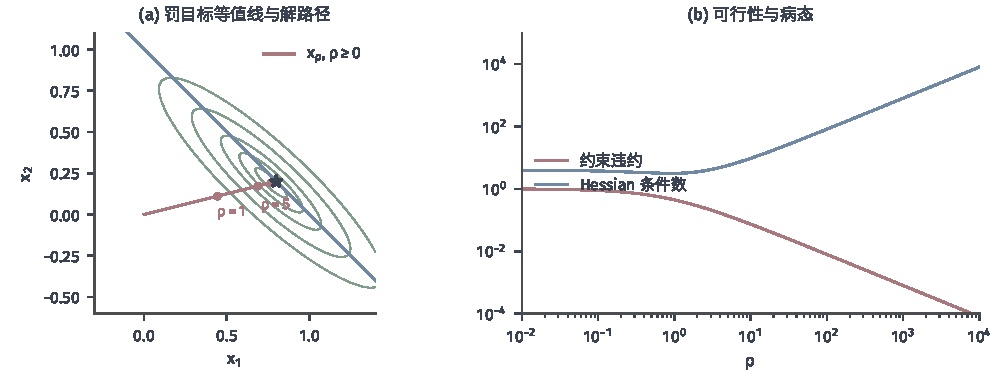
\includegraphics[width=169mm]{figures/03-optimization-evolution-and-signals/01-optimization/matplotlib/c5-penalty-path/figure.pdf}
  \caption{等式二次例的二次惩罚。(a) 绿色椭圆为$\rho=20$时罚目标$Q_\rho$的等值线，沿约束线（蓝）被拉长；红线为解路径$\bm x_\rho=(4\rho,\rho)^\top/(4+5\rho)$，红点标出$\rho=1,5,20$，五角星为约束最优点$(4/5,1/5)^\top$。(b) 对数坐标下，约束违约$4/(4+5\rho)$随$\rho$下降（红），而Hessian条件数（蓝）在$\rho$较大时约按$0.8\rho$增长。}
  \label{fig:opt-con-penalty-path}
\end{figure*}

\subsection{精确惩罚法}
\label{sec:opt-con-exact-penalty}

\paragraph{用违约的绝对值计价}
二次惩罚在可行点附近违约很小时罚得很轻：违约$\delta$只付出$\rho\delta^2/2$，而目标可能因违约获得$|\nu|\delta$量级的好处，所以有限的$\rho$总会接受一点违约。改用违约的一次方计价，
\begin{equation}
\label{eq:opt-con-exact-penalty}
  \Phi_\rho(\bm x)=f(\bm x)+\rho V(\bm x),\qquad
  V(\bm x)=\sum_j|h_j(\bm x)|+\sum_i[g_i(\bm x)]_+,
\end{equation}
小违约的代价与违约成正比，只要单价$\rho$超过目标从违约中获得的边际好处，违约就不划算。以此为目标的方法称为\term{精确惩罚法}（exact penalty method），“精确”的含义是：在适当的有限$\rho$下，惩罚问题的最小点与原问题的最小点对应。代价是$\Phi_\rho$在约束边界上不可微。

图~\ref{fig:opt-con-exact-penalty}用最简单的例子比较两种计价：$\min x$、约束$1-x\leq0$，解$x^\star=1$，乘子$\lambda^\star=1$。二次惩罚$x+\frac\rho2[1-x]_+^2$的最小点是$1-1/\rho$，永远在可行域外。精确惩罚$x+\rho[1-x]_+$在$x<1$时斜率为$1-\rho$：$\rho<1$时目标向左无下界，$\rho=1$时整段$x\leq1$都是最小点，$\rho>1$时唯一最小点就是$x=1$。阈值恰好是乘子。

\begin{figure*}[!htbp]
  \centering
  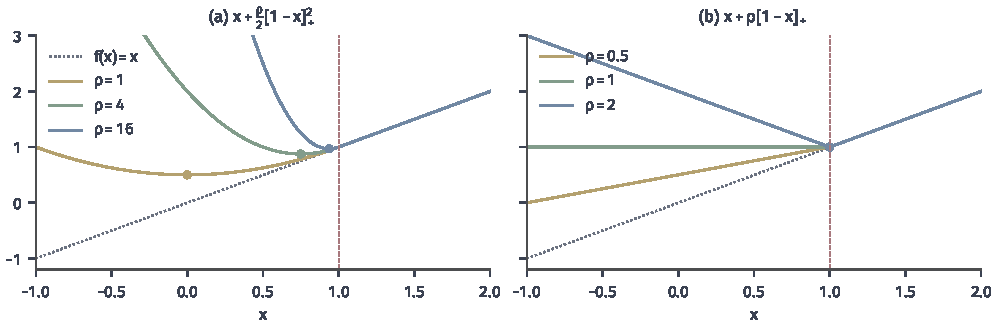
\includegraphics[width=169mm]{figures/03-optimization-evolution-and-signals/01-optimization/matplotlib/c5-exact-penalty/figure.pdf}
  \caption{$\min x$、$1-x\leq0$的两种惩罚，红色竖线为约束边界$x=1$，灰色点线为原目标。(a) 二次惩罚$x+\frac\rho2[1-x]_+^2$，$\rho=1,4,16$时的最小点（圆点）为$1-1/\rho$，都在边界左侧。(b) 精确惩罚$x+\rho[1-x]_+$：$\rho=0.5$时左侧无下界，$\rho=1$时左侧平坦，$\rho=2$时最小点恰为$x=1$。}
  \label{fig:opt-con-exact-penalty}
\end{figure*}

\paragraph{精确性的两条依据}
精确性不是绝对值惩罚的普遍性质，需要条件。第一条依据来自最优乘子。

\begin{theorem}[凸问题的精确惩罚]
\label{thm:opt-con-exact-penalty}
设原问题的强对偶成立，$\bm x^\star$是原问题的最优点，$(\bm\lambda^\star,\bm\nu^\star)$是对偶最优点。若$\rho>\max\{\max_i\lambda_i^\star,\max_j|\nu_j^\star|\}$，则$\bm x^\star$最小化$\Phi_\rho$，且$\Phi_\rho$的每个最小点都可行，因而都是原问题的最优点。
\end{theorem}

\begin{proof}
对任意$\bm x$，$\lambda_i^\star g_i(\bm x)\leq\lambda_i^\star[g_i(\bm x)]_+\leq\rho[g_i(\bm x)]_+$，$\nu_j^\star h_j(\bm x)\leq|\nu_j^\star||h_j(\bm x)|\leq\rho|h_j(\bm x)|$，所以
\[
  \Phi_\rho(\bm x)\geq\mathcal L(\bm x,\bm\lambda^\star,\bm\nu^\star)\geq q(\bm\lambda^\star,\bm\nu^\star)=f(\bm x^\star)=\Phi_\rho(\bm x^\star).
\]
若$\bm x$不可行，则某个$[g_i(\bm x)]_+>0$或$|h_j(\bm x)|>0$，对应项的第二个不等号因$\rho$严格大于乘子而严格成立，$\Phi_\rho(\bm x)>\Phi_\rho(\bm x^\star)$。所以最小点都可行，在可行点上$\Phi_\rho=f$，它们都是原问题的最优点。
\end{proof}

等式二次例中$|\nu^\star|=4/5$，所以$\rho>4/5$时$f+\rho|x_1+x_2-1|$的最小点就是$(4/5,1/5)^\top$。定理只是充分条件，且依赖强对偶与乘子存在；没有这些，绝对值惩罚不必精确。

第二条依据是局部的误差界，它不要求凸性。设在区域$\Omega$内$f$是$K$-Lipschitz的，且每个$\bm x\in\Omega$都有可行点$\bm p\in\Omega$满足$\lVert\bm p-\bm x\rVert_2\leq\kappa V(\bm x)$（违约量控制到可行域的距离）。则
\[
  \Phi_\rho(\bm x)=f(\bm x)+\rho V(\bm x)\geq f(\bm p)-K\kappa V(\bm x)+\rho V(\bm x)=\Phi_\rho(\bm p)+(\rho-K\kappa)V(\bm x),
\]
$\rho>K\kappa$时任何不可行点都严格劣于它的可行修复点，$\Phi_\rho$在$\Omega$中的最小点必可行。这里阈值由误差界常数和Lipschitz常数决定，结论只在$\Omega$内成立。此外，在满足LICQ和二阶充分条件的严格局部最小点处，$\rho$大于乘子的最大绝对值时，该点也是$\Phi_\rho$的严格局部最小点\scite{math-nocedal2006numerical}；这是局部结论，不保证$\Phi_\rho$没有别的更低的局部最小点。

\paragraph{求解与原约束检查}
$\Phi_\rho$非光滑，需要第~\ref{chap:opt-nonsmooth}章的工具：一般情形用次梯度法；违约项有可计算的邻近映射时用邻近梯度法，例如约束只是变量的上下界时，$\rho[x_k-u_k]_++\rho[l_k-x_k]_+$可逐坐标求邻近映射。但$|h_j(\bm x)|$对一般非线性$h_j$不可分，不能套用软阈值公式。不论用哪种方法，返回前都要按原约束重新检查违约，因为数值上只能得到$\Phi_\rho$的近似最小点，而$\rho$是否已越过阈值事先往往未知；若违约不降，就增大$\rho$。

\paragraph{范数正则与范数约束}
机器学习中常见的正则化$\min f(\bm x)+\lambda\lVert\bm x\rVert_1$与约束形式$\min f(\bm x)$、$\lVert\bm x\rVert_1\leq R$有密切关系，但二者不是同一个问题。用本节的语言，前者是把约束$\lVert\bm x\rVert_1-R\leq0$用乘子$\lambda$计价（常数$-\lambda R$不影响最小点）。两个方向都有条件地成立。若约束问题强对偶成立且最优乘子$\lambda^\star$达到，由定理~\ref{thm:opt-con-zero-gap-kkt}(1)，约束问题的每个最优点都最小化$\mathcal L(\cdot,\lambda^\star)=f+\lambda^\star\lVert\cdot\rVert_1-\lambda^\star R$。反过来，若$\hat{\bm x}$最小化$f+\lambda\lVert\cdot\rVert_1$，令$R=\lVert\hat{\bm x}\rVert_1$，则对任意满足$\lVert\bm x\rVert_1\leq R$的$\bm x$，$f(\bm x)\geq f(\hat{\bm x})+\lambda(R-\lVert\bm x\rVert_1)\geq f(\hat{\bm x})$，$\hat{\bm x}$也解约束问题。

但对应关系不是一一的。一维例子$f(x)=\frac12(x-3)^2$：约束$|x|\leq R$的解为$x=\min\{3,R\}$，$0<R<3$时乘子为$3-R$；正则问题的解为软阈值$x=[3-\lambda]_+$。于是$0<R<3$与$0<\lambda<3$之间有$\lambda=3-R$的一一对应，但$R=0$对应全部$\lambda\geq3$，全部$R\geq3$都对应$\lambda=0$。非凸问题中还可能有对偶间隙，此时某些半径根本找不到对应的正则系数。
